\chapter{Introduzione}

\section{Che cos'è l'Internet?}

\dfn{L'Internet}{L'Internet è un sistema che collega molti servizi e dispositivi}

\begin{figure}[h]
\caption{The Internet}
\centering
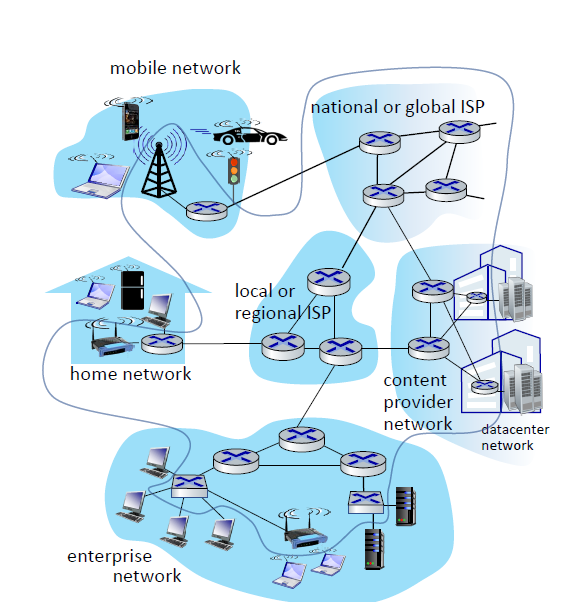
\includegraphics[scale=0.8]{images/Intro/The internet.png}
\end{figure}

\dfn{Apparecchi elettronici}{
\begin{itemize}
    \item Devices: dispositivi connessi a una rete;
    \item Switches: dispositivi che servono per mandare avanti i pacchetti/dati;
    \item Links di communicazione: i componenti che portano i dati da un dispositivo a un altro;
    \item Networks: collegano devices, routers, links, etc.
\end{itemize}
}

\subsection{Che cos'è un protocollo?}

\dfn{Protocollo}{Un protocollo è Un insieme di regole per:
\begin{itemize}
    \item trasferire dati in modo che siano interpretabili;
    \item eseguire specifiche azioni quando si riceve un messaggio o avvengono altri eventi.
\end{itemize}
}

\nt{I protocolli definiscono il formato, l'ordine dei messaggi inviati e ricevuti tra entità del network e le azioni da intraprendere nella trasmissione e nella ricezione dei messaggi}

\begin{figure}[h]
\caption{Protocollo umano vs. Protocollo Internet}
\centering
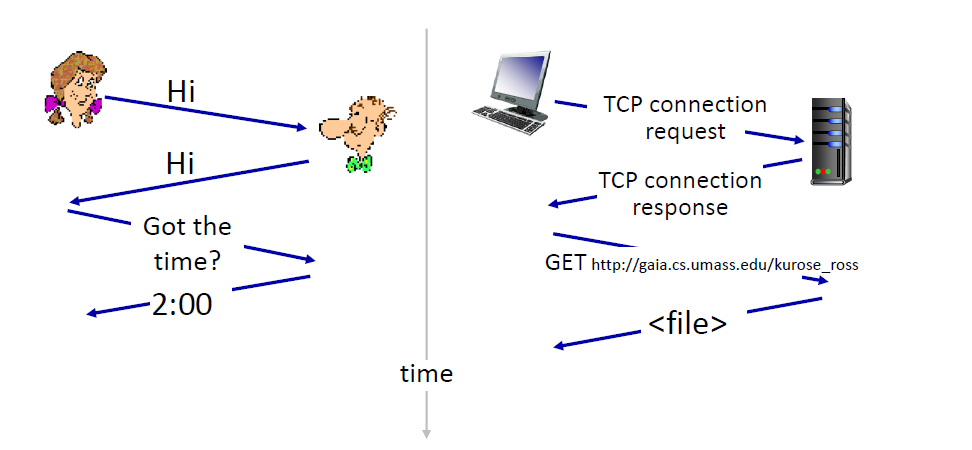
\includegraphics[width=0.8\textwidth]{images/Intro/Protocolli.png}
\end{figure}
\pagebreak
\section{I networks}

\subsection{Access networks}

I cavi possono fare più cose (per esempio trasmettere in TV e accedere a internet). Per fare ciò gli accessi basati su cavo trasmettono su differenti frequenze a seconda del canale (\textit{frequency division multiplexing (FDM)}).

\begin{figure}[h]
\caption{DSL}
\centering
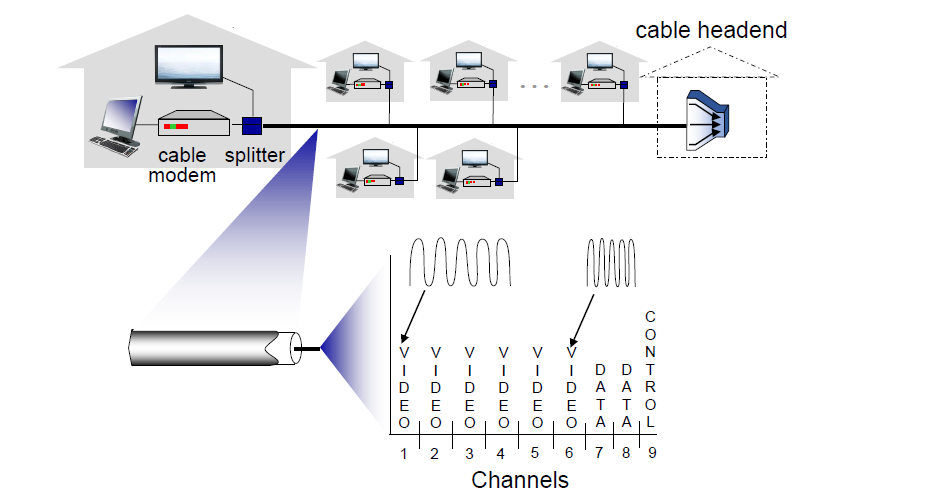
\includegraphics[width=0.8\textwidth]{images/Intro/FDM.png}
\end{figure}

\dfn{HFC}{L'\textit{Hybrid fiber coax(HFC)} era un altro tipo di connessione cablata che aveva un tasso di trasmissione in downstream da 40 Mbps - 1.2 Gbps e in upstream da 30 a 100 Mbps. Questo tipo di tecnologia, al contrario che FDM, è asimmetrica (si usa una via per inviare e una via per ricevere). Il cavo era condiviso.}

\dfn{DSL}{La \textit{Digital subscriber line(DSL)} è una connessione che usa una linea telefonica esistente in cui i dati vanno sulla rete internet e la voce va sulla rete telefonica.}

\pagebreak

\subsection{Home networks}

\dfn{Home network}{In una \textit{home network} ci sono routers, firewalls, access point, etc. Una volta erano tutti separati, attualmente stanno tutti dentro un'unica scatola.}

\begin{figure}[h]
\caption{Home networks}
\centering
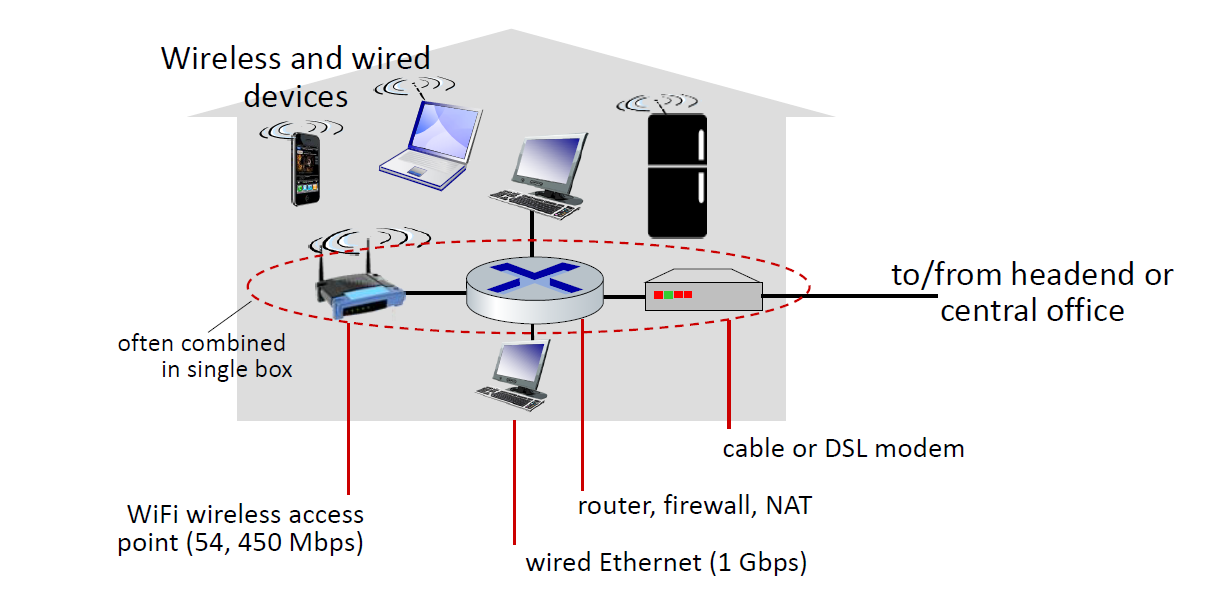
\includegraphics[width=0.8\textwidth]{images/Intro/Home networks.png}
\end{figure}

\subsection{Wireless access networks}

Le frequenze del wireless sono diverse dalle frequenze telefoniche\footnote{In realtà le frequenze del wireless sono le stesse di quelle dei micro-onde}. Sono fatte per comunicazione a corta-media distanza (WLANs, o \textit{Wireless local area networks}) o a lunga distanza (WAN, o\textit{Wide-area cellular access networks}). Il WLANs ha alte frequenze, mentre il WAN a basse frequenze.

\subsection{Enterprise networks}

Sono usate da imprese, università, etc. Sono un mix di tecnologie wired e wireless connessi da routers e switches. Per esempio il wifi e l'ethernet.

\begin{figure}[h]
\caption{Enterprise networks}
\centering
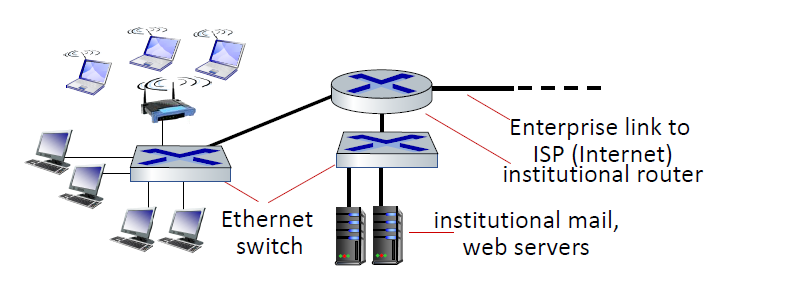
\includegraphics[width=0.8\textwidth]{images/Intro/Enterprise network.png}
\end{figure}

\section{Come si mandano avanti i dati nella rete?}

\nt{Ci sono due tipi di rete: quella \textit{telefonica} (basata sui circuiti) e quella \textit{internet}. Attualmente la rete internet è la più usata.}

\dfn{Pacchetti}{I dati vengono divisi in \textit{pacchetti}, ossia piccole quantità di dati. Ogni singolo pacchetto ha la stessa \textit{lunghezza L}, a eccezione dell'ultimo. Tra il dispositvo e la rete c'è un Linker che ha una determinata \textit{link transmission rate R}.

Il ritardo di trasmissione si calcola come $\frac{L (bits)}{R (bits/sec)}$}

\dfn{Cavi}{
Per trasmettere i dati si possono anche usare dei cavi, che possono essere:

\begin{itemize}
    \item Ethernet;
    \item Coaxial cable: non più usato;
    \item Fibra: ha un'alta velocità e un basso tasso di errore, senza interferenze elettromagnetiche.
\end{itemize}
}

\dfn{Wireless}{Un'altra tipologia di trasmissione è la \textit{wireless} che hanno interferenze, ma non hanno bisogno di un mezzo fisico:

\begin{itemize}
    \item LAN: WiFi;
    \item WLAN: 4G/5G;
    \item NFC: carte di credito contactless;
    \item Bluethooth;
    \item Satellite.
\end{itemize}
}

\section{Il network "core"}

\dfn{Il nucleo dell'Internet}{Il \textit{core} della rete contiene gli ISP che prendono "mandano avanti" i pacchetti (\textit{Forward} o switching). La sua seconda funzione è quella di instradare i pacchetti (\textit{Routing}). Ogni pacchetto contiene un header con la destinazione. Questo header ha un valore che viene inserito in una \textit{Forward table} che indica quale strada prendere.

Il Routing è una scelta globale, il Forward è una scelta locale. L'internet è un grande grafo in cui i percorsi sono individuati dall'\textit{algoritmo di Dijkstra}
}
\pagebreak
\subsection{Il packet-switching}

Si fa \textit{store and forward}, ossia quando arriva un bit del pacchetto viene memorizzato e il pacchetto viene spedito solo quando è arrivato intero. Questo perchè nel pacchetto è scritto il dove inviarlo. Inoltre il pacchetto può essere danneggiato, in questo caso viene scartato.

\begin{figure}[h]
\caption{Packet-switching}
\centering
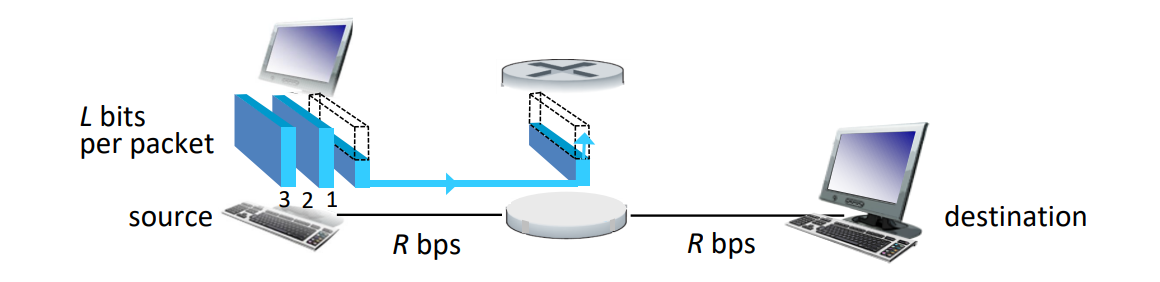
\includegraphics[width=0.8\textwidth]{images/Intro/Packet switching.png}
\end{figure}

\nt{Questo meccanismo causa un ritardo perchè bisogna memorizzare il pacchetto (L/R). Inoltre si può causare traffico. Per risolvere ciò si usa una coda (\textit{queuing}), se diventa troppo lunga si possono scartare i pacchetti (perdita di informazioni). Se la coda è piena si perdono i pacchetti che arrivano. Questo causa la corruzione di programmi, file, ...}

\dfn{TCP}{Il protocollo TCP serve a favorire la trasmissione in tempo reale, per cui se c'è una perdita di informazioni, quando la trasmissione riprende dall'istante attuale e non da quando c'è stato il drop.}

\subsection{Circuit-switching}

Il \textit{circuit-switching} è un'alternativa che crea dei circuiti dedicati tra sorgente e destinazione. Quindi si mandano semplicemente i bit appena arrivano, senza salvarli. Il problema è che per tutta la destinazione si riservano un certo numero di risorse dedicate.

\begin{figure}[h]
\caption{Circuit-switching}
\centering
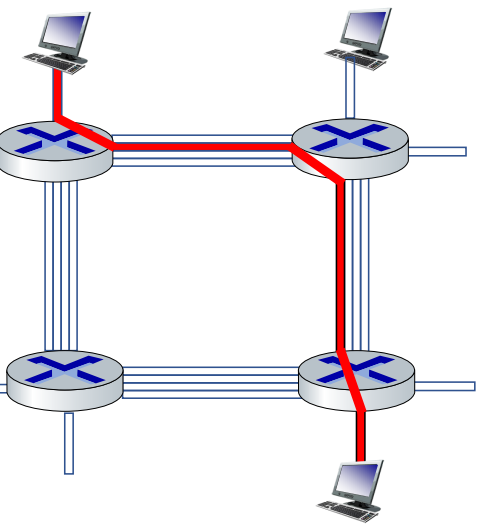
\includegraphics[width=0.4\textwidth]{images/Intro/Circuit switching.png}
\end{figure}

Ci sono due forme di condivisione per riservare le risorse:

\begin{itemize}
    \item Frequency Division Multiplexing (FDM): a ogni utente una frequenza diversa;
    \item Time Division Multiplexing (TDM): a ogni utente un certo lasso di tempo.
\end{itemize}

\begin{figure}[h]
\caption{FDM e TDM}
\centering
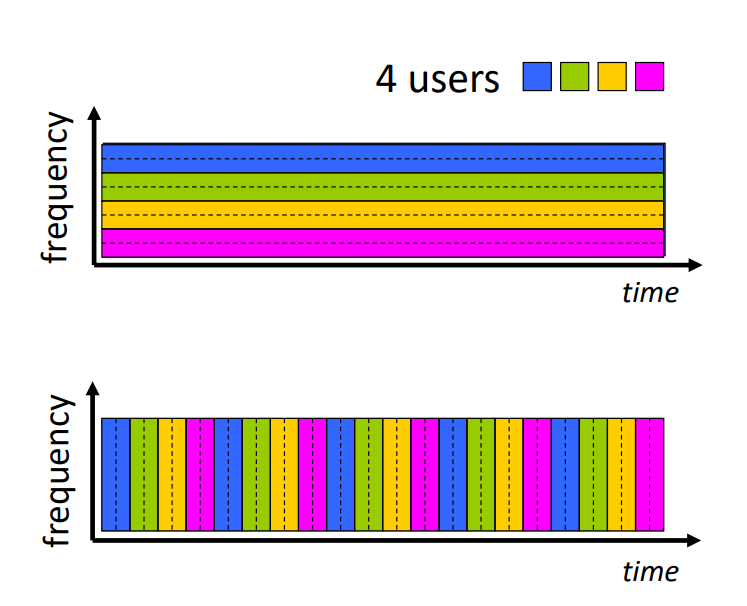
\includegraphics[width=0.4\textwidth]{images/Intro/FDM and TDM.png}
\end{figure}

\nt{ Il packet-switching permette di avere più utenti rispetto al circuit switching. Tuttavia se gli utenti non sono molto attivi questo problema è irrisorio}

\section{Internet structure}

Se si dovessero connettere tutte le reti si avrebbe una complessità O($N^2$), inoltre costerebbe troppo. Ci sono diversi ISP che fanno da connettori collegati tra loro (tramite \textit{peering}, accordi commerciali). Inoltre esistono altre entità, note come \textit{internet exchange point} (IXP) che favoriscono lo scambio di traffico tra i diversi operatori.

\begin{figure}[h]
\caption{Network of networks}
\centering
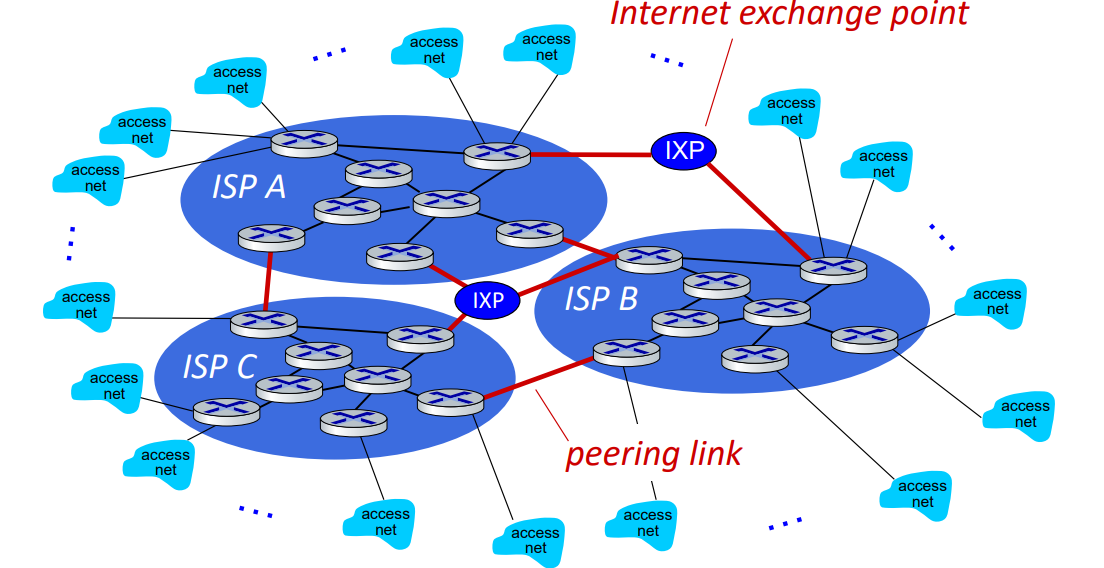
\includegraphics[width=0.6\textwidth]{images/Intro/Network of network.png}
\end{figure}

\dfn{Provider}{I provider possono essere:
\begin{itemize}
    \item Tier 1: NTT, Sprint, AT\&T;
    \item Content provider networks: Google, Facebook.
\end{itemize}
}

\subsection{Le misure di prestazione}

Se si sono mandati un certo numero di pacchetti, quanti se ne sono persi? La perdità deve essere molto bassa.

\qs{}{Quant'è il ritardo?}
\sol{Esso è causato dalla velocità, dal tempo in cui si rimane nella coda, dal tempo di processamento (solitamente bassissimo) e \textit{tempo di propagazione} (lunghezza del link fisico/velocità di propagazione). Per ridurre la latenza si deve fare si che non ci siano code, ridurre il tempo di trasmissione e il tempo di propagazione (portare il pacchetto più vicino).}

\dfn{Traffico e servizio}{
\begin{center}
    $\frac{L * a}{R}$ : $\frac{\text{arrival rate of bits}}{\text{service rate of bits}}$
\end{center}

In questa formula il tasso di arrivo dei bits corrisponde al \textit{traffico} e il tasso di servizio dei bits è l'\textit{intensità}. Mediamente il tasso di arrivo è maggiore al tasso di servizio. Se questo valore è circa 0 c'è un piccolo rallentamento della coda, se è circa 1 c'è un grande rallentamento e se è maggiore di 1 il tempo di attesa tende all'infinito.
}

\dfn{Traceroute e ping}{
La \textit{traceroute} è un programma che serve per misurare i ritardi di un pacchetto nel suo percorso.
Il tracerouter invia tre pacchetti che devono raggiunger il router 'i' durante il loro percorso. Il router 'i' li rispedisce indietro. Chi li ha inviati calcola il tempo impiegato.

IL \textit{ping} permette la verifica dell’effettiva esistenza di un indirizzo IP e controlla che questo sia in grado di accettare delle richieste di comunicazione
}

\nt{  Ogni pacchetto ha un \textit{timeout} che misura quanti dispositivi sono stati attraversati e se si è raggiunto un certo limite "scade" (TTL, Time to live).}

\dfn{Throughput}{Il \textit{Throughput} è la capacità di trasmissione effettiva utilizzata, minore di quella teorica}

\section{Sicurezza nella rete}

\dfn{Sniffing}{}

\dfn{Spoofing}{}

\dfn{DOS}{}

\section{I protocolli}